\documentclass{article}
\usepackage[utf8]{inputenc}
\usepackage[T1]{fontenc}
\usepackage{graphicx}
\usepackage[a4paper]{geometry}
\usepackage{helvet}
\usepackage[pdftex]{hyperref}
\usepackage{pdfpages}
\usepackage{lscape}


\hypersetup{
	pdfauthor={Bruno Lorenz},
	pdftitle={TerrificExporterBundle Documentation},
	colorlinks=true
}

\renewcommand{\familydefault}{\sfdefault}
\renewcommand{\baselinestretch}{1.10}\normalsize

\newcommand{\litem}[1]{
	\vspace{-0.2cm}
	\item{#1}
}


\title{TerrificExporterBundle Documentation}
\author{Bruno Lorenz\\
  Namics AG\\
  Watzmannstraße 1a\\
  81541 München\\
  Germany\\
  \texttt{bruno.lorenz@namics.com}}
\date{\today}

\begin{document}
\tableofcontents



\section{Installation}


% ################################################################################################################################
\subsection{Requirements}
During some functionality is only available since symfony 2.1 it is \textbf{necessary to have your project on a symfony 2.1 basis}. Some actions requires additional tools to do their work. \textbf{As long as this actions are part of the actionstack they will force you to have this tools installed and callable!} If you don't need this action and don't want to install the tools needed for it you have to configure a action stack without this specific action. See chapter '\mbox{\hyperlink{chap-Configuration}{Configuration}}' for more information about defining you own action stack.

% ################################################################################################################################
\subsection{Dependency management}
Update your composer.json and add a new repository. \\

\begin{verbatim}
{
"type" : "vcs",
"url"  : "http://github.com/senuphtyz/TerrificExporterBundle"
}
\end{verbatim}

\noindent After that add a new requirement to your project. \\

\begin{verbatim}
"senuphtyz/terrific-exporter-bundle" : "v2.*"
\end{verbatim}
\noindent Now update your project using the composer. \\

\begin{verbatim}
php composer.phar update
\end{verbatim}
\noindent This should now install alle necessary requirements for your project. \\

% ################################################################################################################################
\subsection{Tooling}
There are a number of tools needed depending on your configuration and tasks.\\

\begin{itemize}
	\litem{YUIDoc}
	\litem{csshint}
	\litem{jslint}
	\litem{jpegoptim}
	\litem{optipng}
	\litem{advpng}
	\litem{montage}
    \litem{diff}
\end{itemize}

\noindent It is necessary to have all tools within path, the exporter won't search for tools on your hardrive. So you have to setup your path variable depending on your os system correctly to have all tools within path's.\\
\\
On Windows: \url{http://www.computerhope.com/issues/ch000549.htm}\\
\\
On *nix/MacOSX: \url{http://www.troubleshooters.com/linux/prepostpath.htm}\\
To do a permanent change it is necessary to change ~/.bashrc or ~/.bash\_profile depending on your os.

% ################################################################################################################################
\subsubsection{YUIDoc, jslint, csshint}
YUIDoc, jslint and csshint are installed using Node.js. Just go to nodejs.org download the package fits for you operating system and install it. \\
After the installation is done open up a new commandline and install Node.js.

\begin{verbatim}
npm -g install yuidocjs jslint csshint
\end{verbatim}

\noindent For further help and syntax for YUIDoc visit \url{http://yui.github.com/yuidoc/}.


% ################################################################################################################################
\subsubsection{jpegoptim, optipng, advpng, montage}

% ################################################################################################################################
\noindent \textbf{Windows}\\
\noindent Jpegoptim is currently not available on Windows systems.\\
\\
Optipng can be retrieved from \mbox{\url{http://optipng.sourceforge.net/}}. Just download the Windows package unzip it no installation required.\\
\\
Advpng or advancecomp can be fetched from \mbox{\url{http://advancemame.sourceforge.net/comp-download.html}}. The same just download and unzip.\\
\\
Montage is part of the ImageMagick toolset. To install ImageMagick visit:\\
\mbox{\url{http://www.imagemagick.org/script/binary-releases.php}} \\

% ################################################################################################################################

\noindent \textbf{Unix/Linux}\\
\noindent On Ubuntu/Debian based Linux it is possible to install jpegoptim directly using your package manager.\\


\begin{verbatim}
sudo apt-get install jpegoptim advancecomp optipng imagemagick
\end{verbatim}

\noindent
On RHEL/Fedora/Centos Linux you have to install jpegoptim from source, rest of the tools could be installed using yum. Download the current version from \url{http://www.kokkonen.net/tjko/projects.html}. \\


\begin{verbatim}
sudo yum install advancecomp optipng ImageMagick
\end{verbatim}

\noindent \textbf{jpegoptim}
\begin{verbatim}
tar zxf jpegoptim-1.2.4.tar.gz
cd jpegoptim-1.2.4
./configure && make && make install
\end{verbatim}


% ################################################################################################################################
\noindent \textbf{MacOSX}\\
\noindent On MacOSX the easiest way to get the whole toolset is to install ImageOptim. This application contains all necessary image optimizing tools needed by the exporter.\\
\\
\url{http://imageoptim.com/}\\
\\
Montage is part of the ImageMagick toolset. To install ImageMagick visit:\\
\url{http://www.imagemagick.org/script/binary-releases.php}\\


% ################################################################################################################################
\subsubsection{diff}

\noindent \textbf{Windows}\\
\noindent On windows there are a number of tools doing the same job as diff on *nixes. You can install a commandline version from diff with \mbox{\href{http://www.cygwin.com/}{cygwin}}.

\noindent \textbf{Unix/Linux}\\
\noindent Normally diff should be installed on all *nixes. If not just install it using your packagemanager. \\
\begin{verbatim}
# Debian/Ubuntu:
sudo apt-get install diff

# RHEL/CentOS/Fedora:
sudo yum install diff
\end{verbatim}

\noindent \textbf{MacOSX}\\
\noindent On MacOSX diff is already installed.



% ################################################################################################################################
\subsection{Setup an export environment}

It is necessary to setup a new environment for you export. To setup an export environment just copy your app/config.yml to app/config\_export.yml. Now you created a new environment called "export". \\
\\
You can now configure the environment to your project needs. For further information visit \url{http://symfony.com/doc/current/cookbook/configuration/environments.html}.\\

\section{Configuration}

All configuration goes beyond a terrific\_exporter node within the config\_export.yml.\\
\\
\textbf{build\_local\_paths: (true/false)}\\
If build\_local\_paths is enabled the exporter will change all urls within html and css files to \\match within the exported package.\\
\\
\textbf{build\_js\_doc: (true/false)} \\
Enables the export of a javascript documentation. The documentation is generated using YUIDoc. \\
\\
\textbf{build\_settings: (path)}\\
This setting should target to a build.ini file. Within this file there are only settings for the \\projektname an versioning data.\\
\\
\textbf{build\_path: (path)}\\
Has to target to a path which is the export target path.\\
\\
\textbf{export\_with\_version: (true/false)}\\
Set to true if the exporter should build zips/folders with version numbers within its name.\\
\\
\textbf{autoincrement\_build: (true/false)}\\
True if the exporter should increase the revision after each build.\\
\\
\textbf{validate\_js: (true/false)}\\
Activates the validation of javascript. Validation is done using jshint.\\
\\
\textbf{validate\_css: (true/false)}\\
Activate the validation of css. Validation is done using csshint.\\
\\
\textbf{optimize\_image: (true/false)}\\
Set to true to optimize images in the output directory. Optimization is done using jpegoptim, \\optipng and advpng.\\
\\
\textbf{export\_views: (true/false)}\\
Activates the export of the views marked with a @Export annotation.\\
\\
\textbf{export\_modules: (true/false)}\\
Activates the export of plain module html. The url within this modules are not rewriten even if \\the build\_local\_paths option is activated.\\
\\
\textbf{export\_type: (string: folder/zip)}\\
Set the export type if the export should be done as folder or as a zip.\\
\\
\textbf{build\_actions: (list of objects)}\\
These option allows to setup a build chain. Here you can append project related exporting tasks or change the buildin order.\\
\\
\textbf{sprites: (list of objects)}\\
Here you can setup sprite information. The exporter will build the sprites with the given data.\\
\\


\subsection{Example configuration}

\begin{verbatim}

terrific_exporter:
	build_local_paths:        true
	build_js_doc:             true
	build_settings:           "build/build.ini"
	build_path:               "build/"
	export_with_version:      false
	autoincrement_build:      true
	validate_js:              false
	validate_css:             false
	validate_html:            false
	optimize_images:          true
	export_views:             true
	export_modules:           true
	export_type:              folder

	build_actions:
	      - Terrific\ExporterBundle\Actions\ClearAction
	      - Terrific\ExporterBundle\Actions\BuildJSDoc
	      - Terrific\ExporterBundle\Actions\ValidateJS
	      - Terrific\ExporterBundle\Actions\ValidateCSS
	      - Terrific\ExporterBundle\Actions\ValidateModules
	      - Terrific\ExporterBundle\Actions\ValidateViews
	      - Terrific\ExporterBundle\Actions\GenerateSprites
	      - Terrific\ExporterBundle\Actions\ExportImages
	      - Terrific\ExporterBundle\Actions\ExportAssets
	      - Terrific\ExporterBundle\Actions\OptimizeImages
	      - Terrific\ExporterBundle\Actions\ExportModules
	      - Terrific\ExporterBundle\Actions\ExportViews

	sprites:
	      - { directory: "PROD/internet_sprite_icons", target: "web/img/sprite_icons.png", item: { height: 50, width: 100 }}

\end{verbatim}
\newcommand{\cmdoptiondesc}[2]{
    \noindent \textbf{#1}\\
    \vspace{-1em}
    \begin{adjustwidth}{\parindent}{0cm}
        #2
    \end{adjustwidth}
    \vspace{1em}
}


\hsection{Usage}

To startup an export use the following command.

\begin{verbatim}
    app/console build:export --env=export --no-debug
\end{verbatim}



\subsection{Commandline options}

\cmdoptiondesc{--no-image-optimization}{
    Overrides configuration setting optimize\_images and starts the chain without optimizing Images. Skip actions:
    \begin{itemize}
          \item{Terrific\textnormal{\textbackslash}ExporterBundle\textnormal{\textbackslash}Actions\textnormal{\textbackslash}OptimizeImages}
    \end{itemize}
}

\cmdoptiondesc{--no-js-doc} {
    Do not build a javascript documentation for this export run. This does skip the following actions:
    \begin{itemize}
        \item{Terrific\textnormal{\textbackslash}ExporterBundle\textnormal{\textbackslash}Actions\textnormal{\textbackslash}BuildJSDoc}
    \end{itemize}
}

\cmdoptiondesc{--no-validation} {
    Ignores validation configuration and skip the following actions:
    \begin{itemize}
          \item{Terrific\textnormal{\textbackslash}ExporterBundle\textnormal{\textbackslash}Actions\textnormal{\textbackslash}ValidateJS}
          \item{Terrific\textnormal{\textbackslash}ExporterBundle\textnormal{\textbackslash}Actions\textnormal{\textbackslash}ValidateCSS}
          \item{Terrific\textnormal{\textbackslash}ExporterBundle\textnormal{\textbackslash}Actions\textnormal{\textbackslash}ValidateModules}
          \item{Terrific\textnormal{\textbackslash}ExporterBundle\textnormal{\textbackslash}Actions\textnormal{\textbackslash}ValidateViews}
    \end{itemize}
}


\subsection{Annotations}

\noindent
\begin{minipage}{\textwidth}
\textbf{@Export}\\
\vspace{-1em}
\begin{adjustwidth}{\parindent}{0cm}
To export a view it is necessary to annotate a controller method with this annotation. It is possible to control a set of options for each view directly within this annotation. This example is only valid if you don't have to export a localized version of a view. If no environment is given this view will exported in all environments.

\begin{verbatim}
 @Export(
     name="viewname.html",
     environment="env1,env2,..."
 )
\end{verbatim}
\end{adjustwidth}
\vspace{1em}
\end{minipage}

\noindent
\begin{minipage}{\textwidth}
\textbf{@LocaleExport}\\
\vspace{-1em}
\begin{adjustwidth}{\parindent}{0cm}
Each view must have their own for each locale which should exported. To set different settings for each locale you have to use the @LocaleExport annotation. This annotation is used in combination with the @Export annotation. Setting up locale exportation will disable exporting the default language which means you have to annotate \textbf{all} locales that should exported. If no environment is given this view will exported in all environments. \\
\\
Usage with @Export:
\begin{verbatim}
@Export(
    @LocaleExport(name="viewname_de.html", locale="de"),
    @LocaleExport(name="viewname_en.html", locale="en", environment="env1"),
    @LocaleExport(name="viewname_lv.html", locale="lv", environment="env2"),
    ....
)
\end{verbatim}
\end{adjustwidth}
\vspace{1em}
\end{minipage}


\hsection{Debugging}

\subsection{Configuration}

\begin{verbatim}
services:
    terrific.formatter.line:
        class: Monolog\Formatter\LineFormatter
        arguments:
            - "[%%datetime%%] [%%level_name%%]: %%message%%\n"

monolog:
    handlers:
        file:
            type:  stream
            path:  %kernel.logs_dir%/%kernel.environment%.log
            level: debug
            formatter: terrific.formatter.line
\end{verbatim}

\noindent
Add this snippet to your export environment configuration.
This snippet will activate logging to a file called like your environment beyond the app/logs directory. The loglevel debug will output a massive amount of logging from the exporter. Currently only the log file contains a list of validation errors for your css / js files. For more information about how to configure your monolog see \url{http://symfony.com/doc/current/cookbook/logging/monolog.html}.
\section{Extending}
\section{Appendix}

\begin{landscape}
    \subsection{Classdiagram}

    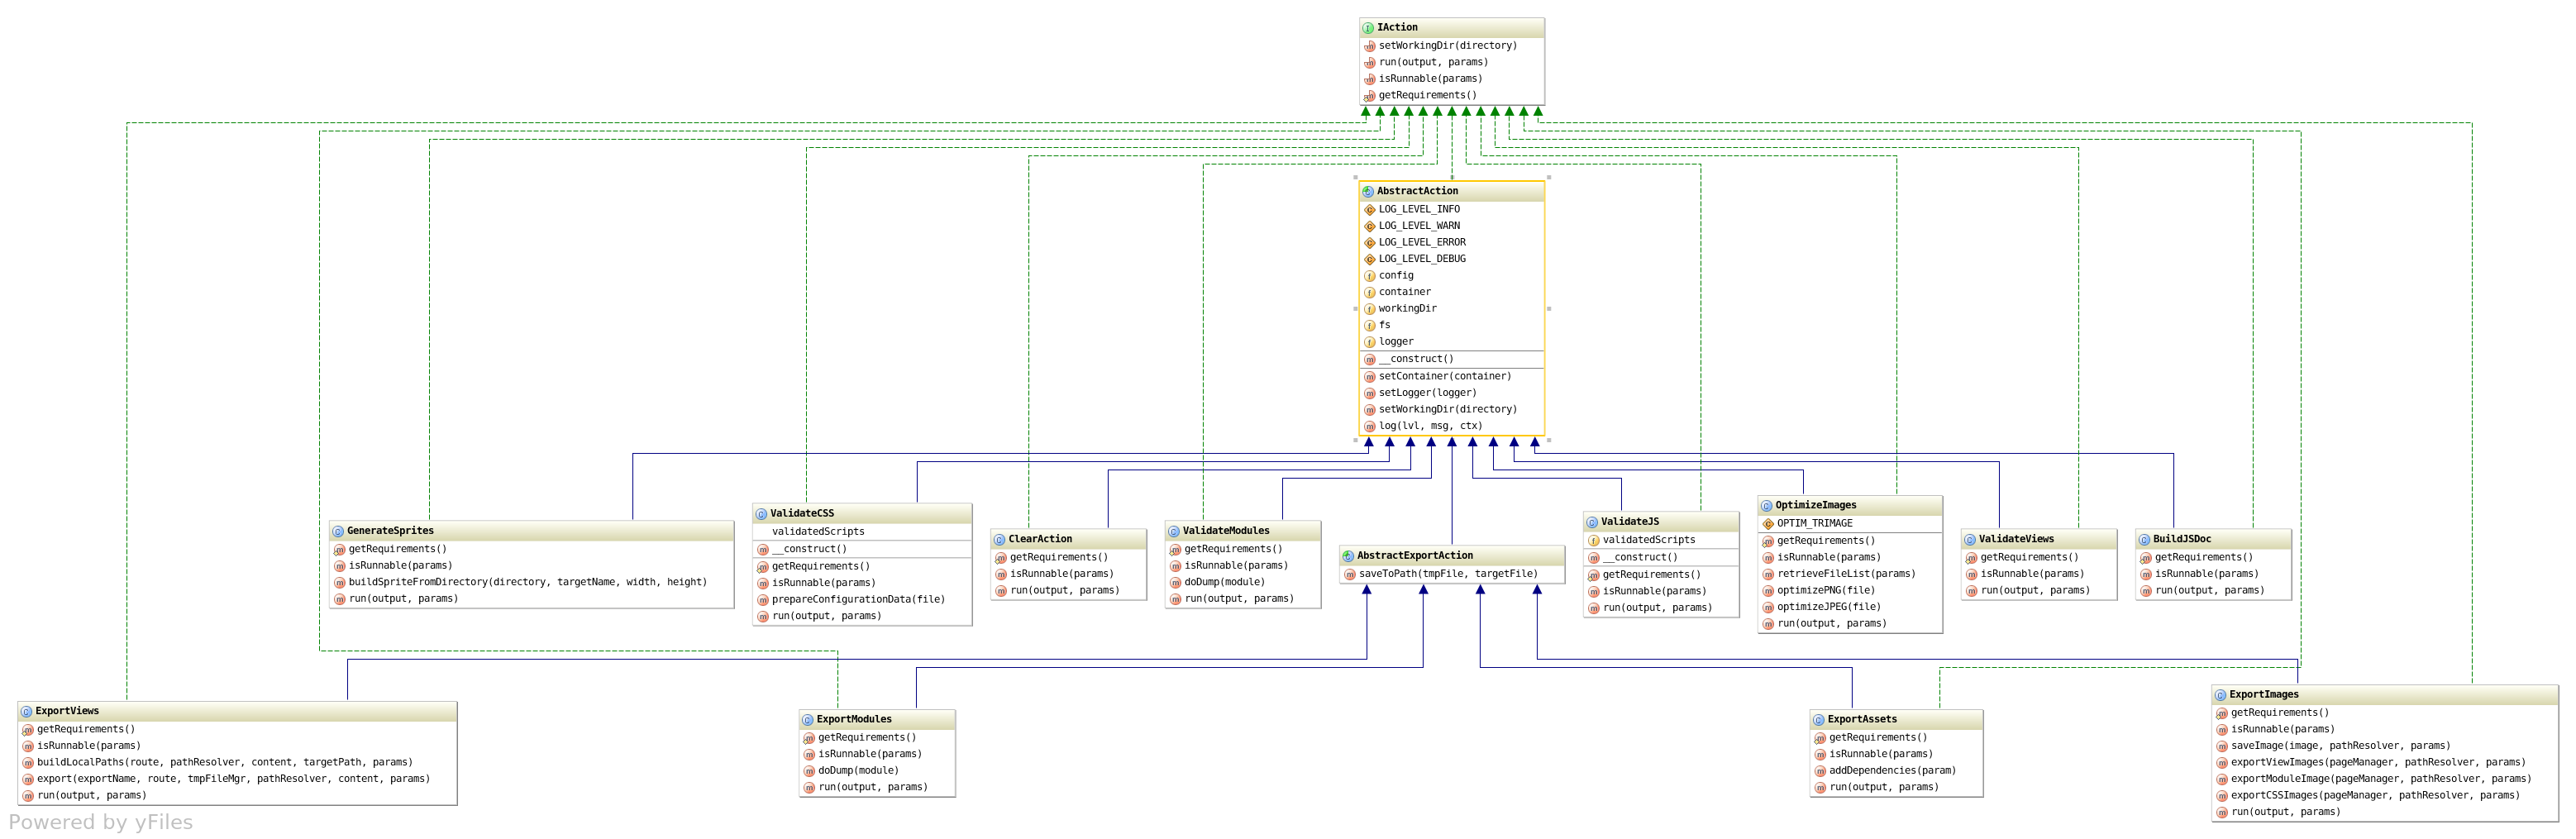
\includegraphics[width=21cm]{diagram.png}
\end{landscape}

\subsection{PHPDocumentation}


\end{document}